\documentclass[journal, letterpaper]{IEEEtran}
%\documentclass{scrartcl}

\usepackage[english]{babel}
%\usepackage[latin1]{inputenc}
\usepackage[utf8]{inputenc}
\usepackage[T1]{fontenc}
\usepackage{amsmath}
\usepackage{amsthm}
\usepackage{amsfonts}
\usepackage{tikz}
\usepackage{verbatim}
\usepackage{subcaption}
\usepackage{algorithm}
\usepackage{algorithmic}
\usepackage[pdftex]{hyperref}

\renewcommand{\algorithmicrequire}{\textbf{Input:}}
\renewcommand{\algorithmiccomment}[1]{\ \ // #1} % C-like // Comments

\hyphenation{render}

% No clubs and widows allowed
\clubpenalty10000
\widowpenalty10000
\displaywidowpenalty=10000
\DeclareMathOperator*{\argmin}{arg\,min}
\begin{document}

%\title{Simulating elastic spheres without external forces}
%\subtitle{Project 1 for class CS6491 Computer Graphics}
\title{Curve Average \\
	{\large Project 3 for class CS6491 Computer Graphics}}
%\author{Sebastian Weiss}
\author{Sebastian Weiss, Can Erdogan \\ \today}
%\date{\today}

\maketitle

\begin{tikzpicture}[remember picture,overlay]
   \node[anchor=north east,inner sep=0pt] at (current page.north east)
              {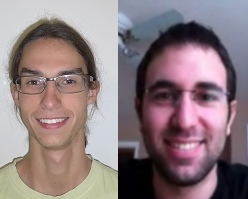
\includegraphics[scale=1.5]{pic}};
\end{tikzpicture}

\section{Objective}
Formally, for two curves $A = \{a_0 ... a_{n-1}\}$ and $B = \{b_0 ... b_{n-1}\}$, each with $n$ points and $\forall x \in (A \cup B), x \in \mathcal{R}^3$,
the goal is to find a curve $C$ such that for each point $c \in C$, and its closest projections
\begin{align}
a^c &= \operatornamewithlimits{argmin}\limits_{a \in A} ||a-c|| \text{, and} \\
b^c &= \operatornamewithlimits{argmin}\limits_{b \in B} ||b-c||
\end{align}

\noindent the following holds true:

\begin{equation}
 c = \operatornamewithlimits{argmin}\limits_{x \in L(a^c, b^c)} ||a^c-x||
\end{equation}

\noindent where for each point $r$ on line $L(p,q)$, $||r-p|| = ||r-q||$. Moreover, for
any three consecutive sampled points $c_i$, $c_j$ and $c_k$ on curve $C$, the arc lengths
of the curves between their closest projections are the same:
\begin{equation}
\small
 D^A(a^{c_i},a^{c_j}) + D^B(b^{c_i},b^{c_j}) = D^A(a^{c_j},a^{c_k}) + D^B(b^{c_j},b^{c_k})
\end{equation}
\noindent where $D^Z(x,y)$ is the distance along the curve $Z$ between points $x,y \in Z$.

Semantically, we want to find the curve that is composed of the loci of the smallest spheres that touch the two inputs curves A and B,
and sample it such that for each sample on the curve, the distances traveled by the matching samples along their curves is a constant.

\section{Input}
The input is the six control points for two curves $A$ and $B$, named $A_0$ to $A_5$ and $B_0$ to $B_5$, such that the first and the last control points are the same.

\section{Overview}
The project is composed of the following three main parts: (1) the representation of the curves,
(2) the computation of the average curve, and (3) the visualization of the different curve properties.
The challenge in the representation is that we want the spline curves to first meet at two end points and then,
to have $C^1$ continuity at the intersection of the splines. For the curve average, we had to ensure
the points satisfied the constraints in Equations 1-3. Lastly, the visualization contained multiple challenges
including parallel transport, circular arc computation and etc.

\section{Curve Representation}
We compose each curve out of piecewise quadratic Hermite and cubic Hermite splines. Each spline is connected at a control point by the same local velocity. This leads to a $\mathcal{C}^1$-smooth curve.
We define the tangent/velocity at control point $A_i$ as $T_i = c*(A_{i+1}-A_{i-1})$. The parameter $c$ defines the curvature or the influence of that velocity. In our experiments, we set $c$ to 0.5.

A cubic Hermite spline requires velocities at both end points, a quadratic Hermite spline only at one end point. Therefore, we use the quadratic form for the first and the last part of the curve and the cubic form for all middle parts.

\subsection{Quadratic Hermite Spline}
Given the points $X_0$ and $X_1$ and the tangent $T_0$, find a quadratic spline $P(t)$ so that the following holds:
\begin{equation}
\small
 P(0)=X_0, P(1)=X_1, P'(0)=T_0
\end{equation}
Solving this system of equation leads to the following formula:
\begin{equation}
\small
 P(t) = (t^2-2t+1)X_0 + (-t^2+2t)X_1 + (t^2-t)T_0
\label{eq:QuadraticHermite}
\end{equation}

\subsection{Cubic Hermite Spline}
Given the points $X_0$ and $X_1$ and the tangents $T_0$ and $T_1$, find a cubic spline $P(t)$ so that the following holds:
\begin{equation}
\small
 P(0)=X_0, P(1)=X_1, P'(0)=T_0, P'(1)=T_0
\end{equation}
This equation is solved similar to the quadratic case, leading to:
\begin{equation}
\small
 P(t) = (2t^3-3t^2+1)X_0 + (t^3-2t^2+t)T_0 + (-2t^3+3t^2)X_1 + (t^3-t^2)T_1
\label{eq:CubicHermite}
\end{equation}

\section{Average Curve Computation}

\subsection{Distance functions}
TODO

\subsection{Curve tracing}
TODO

\subsection{Average Distance (geodesic) Sampling}
TODO

\section{Visualization and Editing}

\begin{figure*} %This just must appear at the page before the chapter "Displaying the average curve"
	\centering
		\begin{tabular}{cccc}
			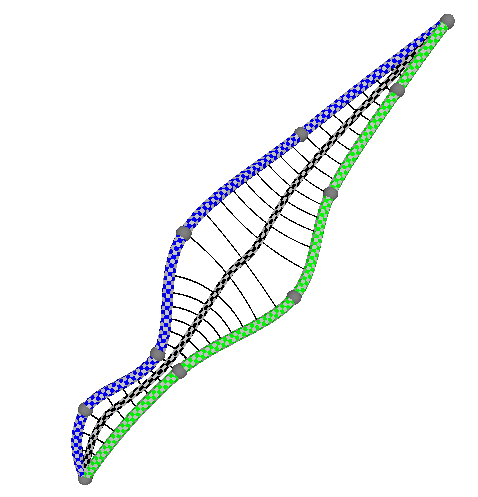
\includegraphics[scale=0.4]{images/NoGeodesicSampling.png} & 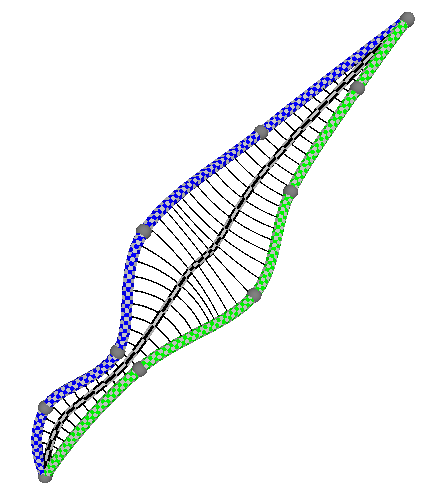
\includegraphics[scale=0.4]{images/GeodesicSampling.png} 
				& 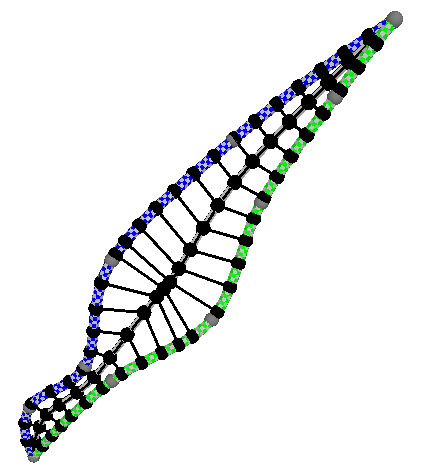
\includegraphics[scale=0.4]{images/ClosestProjections.png} & 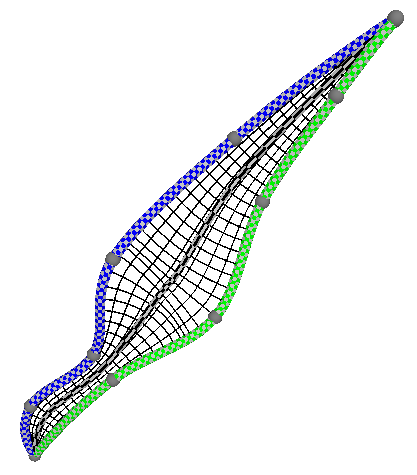
\includegraphics[scale=0.4]{images/CircularArcNet.png} \\
			\small
			a) no geodesic sampling & b) with geodesic sampling & c) the closest projections & d) net of circular arcs
		\end{tabular}
	\caption{Geodesic sampling, closest projections and circular arcs}
	\label{fig:GeodesicSampling}
\end{figure*}

We provide a framework for editing the control curve and visualizing the curve average.
More specific, we support the following features: 
\begin{itemize}
	\item Moving the control points of the two input curve
	\item Displaying the curve average with or without geodesic sampling
	\item Displaying the closest projections
	\item Displaying the circular arc and animating the curve average along it
	\item Showing the inflation tube, the envelope of the smallest spheres
\end{itemize}
We now describe the single features in more detail

\subsection{Editing and displaying the control curve}
We display the control points as gray spheres and the two control curves in green and blue.
The user can click the control points and change their positions by dragging them over the screen.

\subsection{Displaying the average curve}
The curve average is displayed by connecting the sample points using piecewise straight tubes. The faces of the tubes are rendered in alternating black and gray so you can see where the trace points are.
The user has now the option to toggle geodesic sampling on or off. The effects are shown in Fig.\ref{fig:GeodesicSampling}ab. 

As you can see, without geodesic sampling, the distances between the samples of the curve average are almost equispaced, but the closest projections on the control curve, indicated by the circular arcs, vary greatly in the distances. With geodesic sampling turned on, the curve average is sampled in that way that the sum of the distances between two consecutive closest projects on the control curves are constant. However, this leads to large variation of the distances of the curve average samples.

\subsection{Closest projections}
To visualize the closest projections, i.e. the points on the control curve that are closest to the average curve at this point, we draw straight lines between the sample of the curve average and its closest projections. These can be seen in Fig.\ref{fig:GeodesicSampling}c. Note that the lines to both control curves are of the same length and that they stand orthogonal to the control curve at the intersections. These are the properties that define the closest projections and the curve average.

\subsection{Circular arc}
Instead of displaying the closest projections as straight lines, we could also draw them using circular arcs.
\begin{figure}[ht!] 
  \centering
	\begin{tikzpicture}[scale=0.5]
		\coordinate[label=right:P] (P) at (0,0);
		\coordinate[label=left:A] (A) at (-6,-2);
		\coordinate[label=right:B] (B) at (6,-2);
		\coordinate[label=right:C] (C) at (0,-20);
		\draw (P)--(A); %closest projections
		\draw (P)--(B);
		\draw[blue,thick] (6.4,-0.8) coordinate -- (5.6,-3.2) coordinate; %parts of the control curve
		\draw[green,thick] (-6.4,-0.8) coordinate -- (-5.6,-3.2) coordinate;
		\draw (-6.2,-1.4) coordinate -- (-5.6,-1.2) coordinate -- (-5.2,-2.4) coordinate -- (-5.8,-2.6) coordinate; % right angles
		\draw (6.2,-1.4) coordinate -- (5.6,-1.2) coordinate -- (5.2,-2.4) coordinate -- (5.8,-2.6) coordinate;
		\path[blue,thick] (6.4,-0.8) coordinate edge[out=70,in=-120] (6.8,1) coordinate; % control curve
		\path[blue,thick] (5.6,-3.2) coordinate edge[out=250,in=100] (5.8,-5) coordinate;
		\path[green,thick] (-6.4,-0.8) coordinate edge[out=110,in=-120] (-7,1) coordinate;
		\path[green,thick] (-5.6,-3.2) coordinate edge[out=290,in=80] (-5,-5) coordinate;
		\path[black,thick] (0,0) coordinate edge[out=90,in=-70] (-0.2,1) coordinate; % average curve
		\path[black,thick] (0,0) coordinate edge[out=-90,in=110] (0.2,-3) coordinate;
		\draw (A)--(C); %circle sides
		\draw (B)--(C);
		\coordinate[label=left:r] (r) at (-4,-8);
		\draw[red,thick] ([shift=(71.567:19)] 0,-20) arc (71.567:108.435:19); %circular arc
		\tikzset{mypoints/.style={fill=white,draw=black,thick}} %coordinate points
		\fill[mypoints] (P) circle (5.0pt);
		\fill[mypoints] (A) circle (5.0pt);
		\fill[mypoints] (B) circle (5.0pt);
		\fill[mypoints] (C) circle (5.0pt);
	\end{tikzpicture}
	\caption{circular arc}
	\label{fig:CircularArc}
\end{figure}
In Fig.\ref{fig:CircularArc}, you can see parts of the two input curves in green and blue and the curve average in black in the middle. The current trace point is $P$ and the closest projections of $P$ on the control points are $A$ and $B$. \\
We can now construct a unique circle in 3d with center $C$, radius $r$ and normal $N$ that goes through $A$ and $B$ and the tangents at these points are $AP$ and $BP$.

First, assume $A$,$B$,$P$ are not collinear. Then $ABP$ defines a plane with the normal vector $N=\underline{PA} \times \underline{PB}$. The circular arc lies in that plane. The vectors $U=N \times \underline{PA}$ and $V=N \times \underline{PB}$ are normals of the circle at these points.
Therefore, the rays $A+\alpha U$ and $B+\beta V$ intersect exactly at the circle center $C$.
This system is overdetermined but we can solve for $\alpha$ in the following way:
\begin{equation}
\begin{array}{rcl}
A + \alpha U &=& B + \beta V \\
\alpha U &=& B-A+\beta V \\
(\alpha U) \times V &=& (AB+\beta V) \times V \\
\alpha (U\times V) &=& (AB) \times V
\end{array}
\label{eq:CircArc}
\end{equation}
And now we have $\alpha = \frac{ ((AB)\times V).x }{ (U \times V).x}$. We can pick any coordinate, all have to be the same.

This then leads to $C=A + \alpha U$, $r=|AC|$ and $N$ as described above.

If the points $A$,$B$,$P$ are collinear, indicated by $N=0$ (plus epsilon), then the circular arc degenerates to a linear interpolation (lerp) from A to B through P.

We draw the circular arc by approximating it using piecewise straight tubes. The samples are obtained by rotating the vector $CA$ around $N$ until it becomes $CB$. This is done the same way as in the Swirl-project:
\begin{equation}
\begin{array}{lcl}
 CA^{\circ}(\theta; N) &:=& C + U^{\circ}(\alpha; N) \\
                        & =& C + \cos \alpha U - \sin \alpha (N \times U)\\
 \multicolumn{3}{l}{\text{with } V := CA\angle\underline{N} = (W\bullet\underline{N})\underline{N}} \\
 \multicolumn{3}{l}{\text{and } U = CA-V} \\
 \multicolumn{3}{l}{\theta \text{ ranges from } 0 \text{ to } CA^{\wedge}CB=\cos^{-1}(\underline{CA}\bullet\underline{CB})}
\end{array}
\label{eq:Rot}
\end{equation}

Furthermore, if we sample the circular arcs at some angles and combine the samples with the same angle, we obtain a net, as shown in Fig.\ref{GeodesicSampling}d. If both control curves lie in a plane, this net also lies in the same plane.

We further provide the ability to animate the average curve between the two control curves. In that animation, each sample of the average curve follows the circular arc between the closest projections.

\subsection{Inflation tube}
\begin{figure}
	\centering
		\begin{tabular}{ccc}
			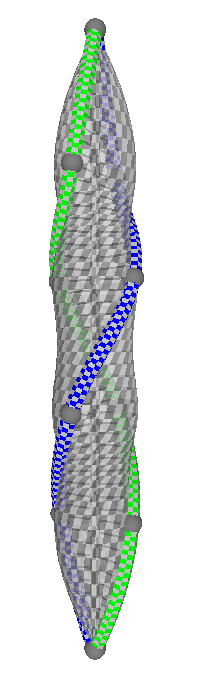
\includegraphics[scale=0.7]{images/InflationNoParallelTransport.png} & 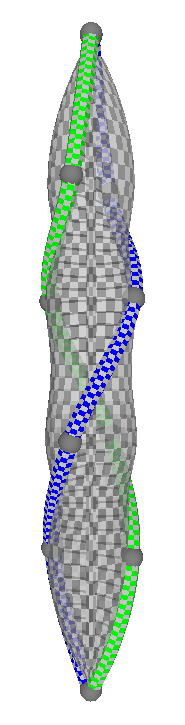
\includegraphics[scale=0.7]{images/InflationParallelTransport.png} 
				& 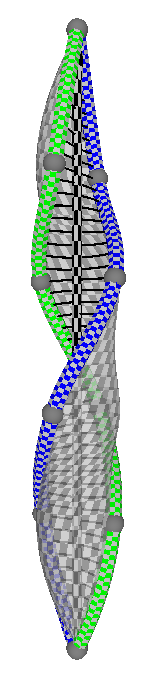
\includegraphics[scale=0.7]{images/InflationHalf.png}\\
			a) no  & b) with & c) \\
			parallel transport & parallel transport & half tube
		\end{tabular}
	\caption{the inflation tube}
	\label{fig:Inflation}
\end{figure}
As a last graphic feature, we draw the inflation tube. The inflation tube is the envelope of the minimal balls along the curve average.
It can be seen as the union of all balls with the center on the curve average that exactly touches the control curve and contains no other point in the interior.

\subsubsection{Drawing the inflation tube}

To draw the inflation tube, we get the following input from the tracing algorithm: the samples of the average curve $P_i$, $i\in\{0,...n-1\}$, the closest projections on the two control curves $A_i$ and $B_i$ and the radii or distances to the closest projections $r_i$. We further define the tangent $T_i$ at the average curve sample $i$ as $T_i=\frac{1}{2}(P_{i+1}-P_{i-1})$.

The first way one might think of drawing it, is to circles around the average curve samples $P_i$ in the plane orthogonal to the tangents $T_i$ with radii $r_i$ and connect them to tubes. However, this approach will lead to wrong results since the closest projections to the control curves are not orthogonal to the average curve tangent. Therefore, the distance from the closest projections to the average curve is not equal to the radius of the circle when it should touch the control curves.\\

We present a different approach now. Instead of drawing circles orthogonal to the tangents, we directly take the vectors $P_i A_i$ and rotate them around $T_i$. This technique is visualized in Fig.\ref{fig:InflationDrawing}. We rotate $P_i A_i$ as described in Eq.\ref{eq:Rot} the whole $360^{\circ}$. At $180^{\circ}$, the vector becomes $P_i B_i$. We then sample the circles at constant angles and connect samples with the same angle, leading to the tube as shown in Fig.\ref{fig:Inflation}a.

\begin{figure}[ht!] 
  \centering
	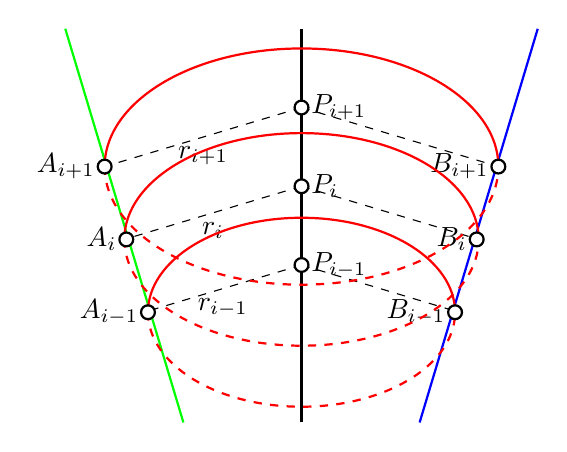
\begin{tikzpicture}[scale=0.5]
		\draw[black,thick] (0,0) coordinate -- (0,10) coordinate; %curves
		\draw[green,thick] (-3,0) coordinate -- (-6,10) coordinate;
		\draw[blue,thick] (3,0) coordinate -- (6,10) coordinate;
		\coordinate[label=right:$P_{i+1}$] (P2) at (0,8) coordinate; %samples
		\coordinate[label=right:$P_{i}$] (P1) at (0,6) coordinate;
		\coordinate[label=right:$P_{i-1}$] (P0) at (0,4) coordinate;
		\draw[dashed] (0,8) coordinate -- (5,6.5) coordinate; %closest projections
		\draw[dashed] (0,8) coordinate -- (-2.5,7.25) coordinate node[below] {$r_{i+1}$} -- (-5,6.5) coordinate;
		\draw[dashed] (0,6) coordinate -- (4.5,4.65) coordinate;
		\draw[dashed] (0,6) coordinate -- (-2.25,5.325) coordinate node[below] {$r_{i}$} -- (-4.5,4.65) coordinate;
		\draw[dashed] (0,4) coordinate -- (4,2.8) coordinate;
		\draw[dashed] (0,4) coordinate -- (-2,3.4) coordinate node[below] {$r_{i-1}$} -- (-4,2.8) coordinate;
		\coordinate[label=left:$A_{i+1}$] (A2) at (-5,6.5) coordinate; %closest projection points
		\coordinate[label=left:$A_{i}$] (A1) at (-4.45,4.65) coordinate;
		\coordinate[label=left:$A_{i-1}$] (A0) at (-3.9,2.8) coordinate;
		\coordinate[label=left:$B_{i+1}$] (B2) at (5,6.5) coordinate;
		\coordinate[label=left:$B_{i}$] (B1) at (4.45,4.65) coordinate;
		\coordinate[label=left:$B_{i-1}$] (B0) at (3.9,2.8) coordinate;
		\draw[red,thick] ([shift=(180:5)] 0,6.5) arc (180:0:5 and 3); %tube elipses
		\draw[red,dashed,thick] ([shift=(180:5)] 0,6.5) arc (180:360:5 and 3);
		\draw[red,thick] ([shift=(180:4.5)] 0,4.65) arc (180:0:4.5 and 2.7);
		\draw[red,dashed,thick] ([shift=(180:4.5)] 0,4.65) arc (180:360:4.5 and 2.7);
		\draw[red,thick] ([shift=(180:3.9)] 0,2.8) arc (180:0:3.9 and 2.4);
		\draw[red,dashed,thick] ([shift=(180:3.9)] 0,2.8) arc (180:360:3.9 and 2.4);
		\tikzset{mypoints/.style={fill=white,draw=black,thick}} %coordinate points
		\foreach \p in {P0,P1,P2,A0,A1,A2,B0,B1,B2}
			\fill[mypoints] (\p) circle (5.0pt);
	\end{tikzpicture}
	\caption{inflation tube}
	\label{fig:InflationDrawing}
\end{figure}

\subsubsection{Parallel transport}
When the control curves rotate around the average curve, the inflation tube follows this rotation, as seen in Fig.\ref{fig:Inflation}a. However, often Fig.\ref{fig:Inflation}b is required. Here, the rotation of the inflation tube stays constant although the control curves rotate around it.

The technique to achieve this result is called Parallel Transport. The only thing we have to do is to modify the start angle $\alpha_i$. Instead of sampling each circle (see previous section) starting with $0^{\circ}$, we start it at an angle that minimizes the rotation to the previous circle.

The task is now the following: given the previous tangent $\underline{T_{i-1}}$, rotated vector $P_{i-1}A_{i-1}$ and start angle $\alpha_{i-1}$, and the current tangent $\underline{T_i}$ and rotated vector $P_i A_i$, find the current start angle $\alpha_i$ so that the twist is minimized.
In other words, we have to find $\alpha_i$ so that $P_i A_i^{\circ}(\alpha_i; T_i)$ lies in the plane spanned by $T_{i-1}$ and $X:=P_{i-1}A_{i-1}^{\circ}(\alpha_{i-1}; T_{i-1})$:

\begin{equation}
	\begin{array}{rcl}
		\underline{X} &:=& \underline{P_{i-1}A_{i-1}^{\circ}(\alpha_{i-1}; T_{i-1})} \\
		\underline{N'} &:=& \underline{T_{i-1}} \times \underline{X} \\
		\underline{PA'} &:=& \underline{P_i A_i} \\
		x &:=& \underline{PA'} \bullet \underline{N'} \\
		y &:=& \underline{PA'} \bullet \underline{X} \\
		PA'' &:=& xN' + yX \\
		\alpha_i &:=& ( (x<0)?(-1):1 ) \cdot \cos^{-1}(\underline{X} \bullet \underline{PA''})
	\end{array}
\label{eq:ParallelTransport}
\end{equation}
$\underline{N'}$ is the normal of the reference plane, then we project $P_i A_i$ in that plane and obtain $PA''$. The final angle $\alpha_i$ is then the angle between the reference vector $X$ and the projected vector $PA''$. Since this angle does not include the direction of the twist, we have to invert the angle if $x<0$.

\subsubsection{half tube}
Instead of drawing the whole inflation tube without parallel transport, we could also draw only half of it. This leads to the interesting effect of a waterslide as seen in Fig.\ref{fig:Inflation}c.

\section{Results}
In conclusion, we are able to trace the average curve of two piecewise hermite interpolated curves in real-time, whereat the user defines the control points by dragging them around.
We presented ideas on how to detect if the two control curves are compatible or not.
Furthermore, we showed different ways on how to display the average curve, using line segments to the closest projections, circular arcs or the inflation tube.

\section{Future work}
This work can easily be extended to any kind of input curve and any number of control points.
Also more freedom for the user to specify the input curve, like editing the velocities, might be helpful for specific applications.

% EXAMPLES
\begin{figure*}
	\centering
		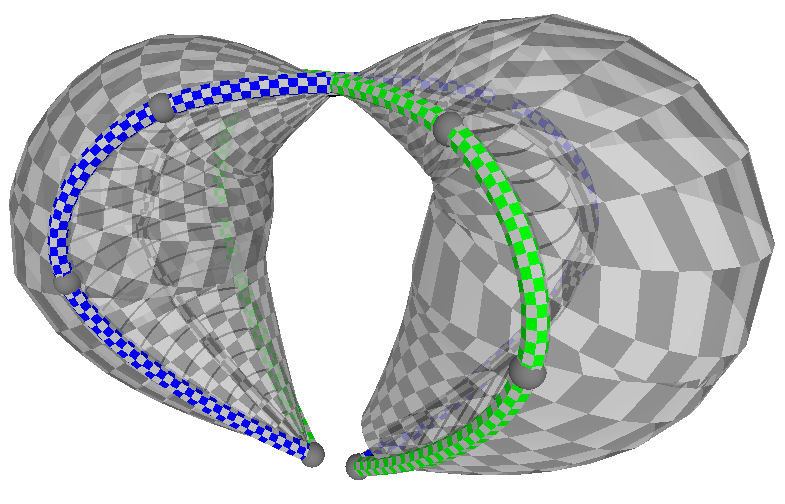
\includegraphics[scale=0.4]{images/Result1.png}
		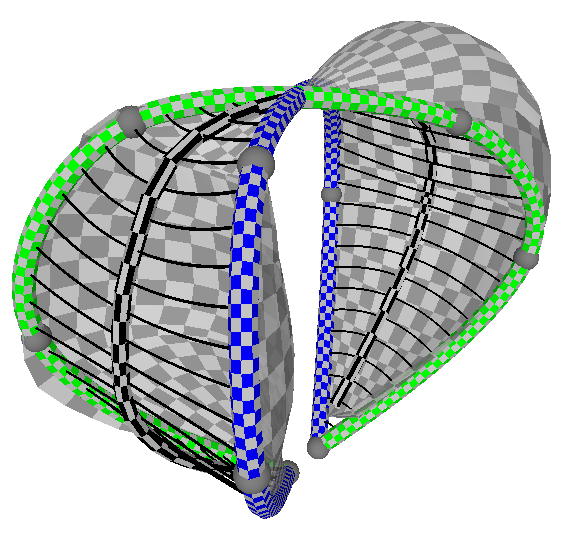
\includegraphics[scale=0.4]{images/Result2.png}
	\caption{Example 1: a bow}
	\label{fig:Result1}
\end{figure*}
\begin{figure*}
	\centering
		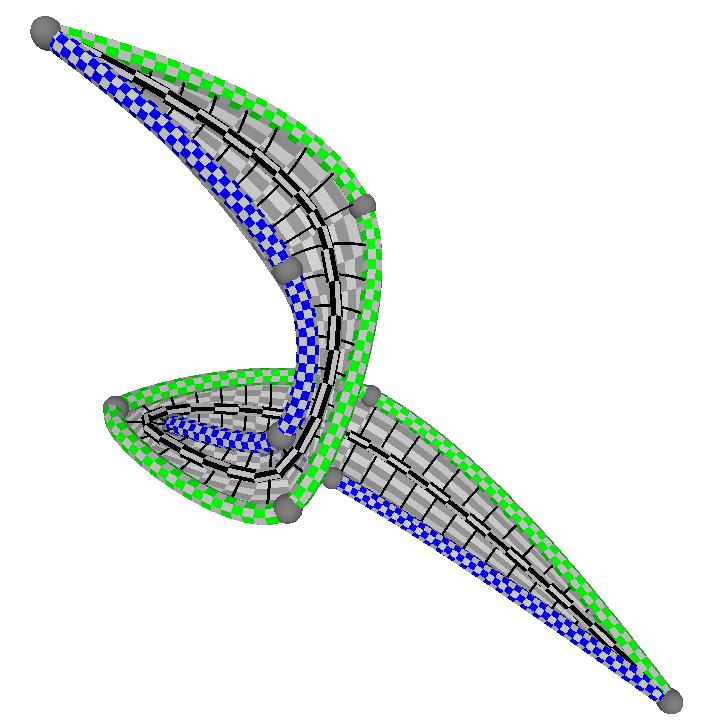
\includegraphics[scale=0.4]{images/Result3.png}
	\caption{Example 2: a waterslide}
	\label{fig:Result3}
\end{figure*}
\begin{figure*}
	\centering
		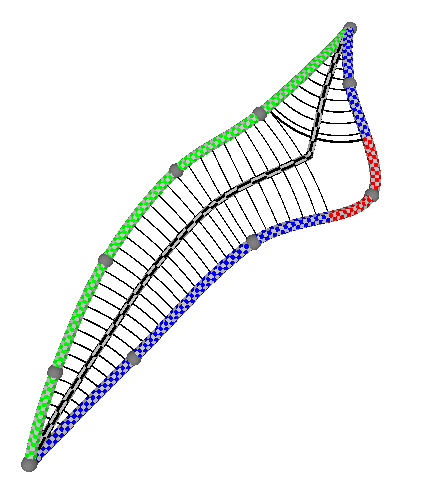
\includegraphics[scale=0.5]{images/Result4.png}
		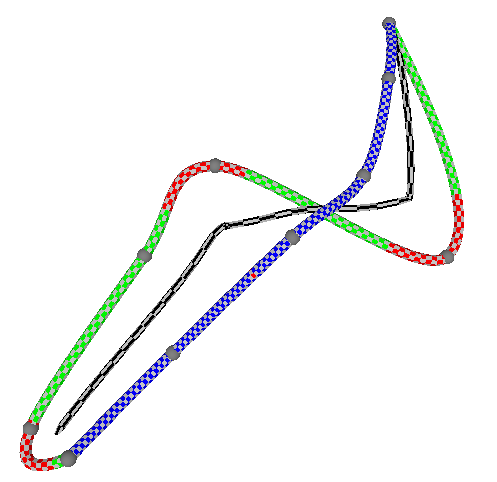
\includegraphics[scale=0.5]{images/Result5.png}
	\caption{Example 3: extreme cases and non-compatibility detection}
	\label{fig:Result4}
\end{figure*}

\end{document}